% Chapter 3

\chapter{Lexical and superlexical prefixes?} 
\label{Chapter4}
%\lhead{Chapter 3. \emph{Lexical and \isi{superlexical} prefixes?}} % 
%The theoretical advances described in \ref{Chapter2} rule out a lot of impossible combinations of prefixes and makes the whole picture of Russian \isi{prefixation} much more clear, but the following questions still remain unanswered:
%\begin{itemize}
%\item Why this or that prefix in a particular meaning falls in one or another group?
%\item Why the same prefixes with different meaning end up in different groups? Is there a theory-\isi{external} explanation for this?
%\item Do the prefixes belonging to one group behave uniformly?
%\item Are that all the impossible combinations ruled out by the theory?
%\item Are all the combinations allowed predicted to be such by the theory?
%\end{itemize}
%As several researches have pointed out the problems with the \isi{superlexical}/lexical distinction, I will start with an overview of the main points concerning this topic and continue with discussing the questions formulated above. 

%\section{Lexical and superlexical prefixes}\label{section:new:distinction}
This chapter discusses in detail the distinction between lexical and \isi{superlexical} prefixes. This opposition constitutes the main driving force of the syntactic approaches to Russian \isi{prefixation} (\citealt{Ramchand:04, Svenonius:04b, Romanova:06}, among others), as prefixes that belong to different groups are claimed to have distinct \isi{syntactic positions} and properties. In what follows I provide details about the history and various refinements of this distinction and discuss problems it involves. I then show that neither the bipartite nor the more fine-grained distinctions are sufficient to account for the full range of data. Based on the observations about the vagueness of the distinction together with insufficient predictive power, I abandon the hypothesis that the formation of \isi{complex verbs} depends primarily on the structural positions of the affixes and develop an alternative (semantic) approach in Chapter~\ref{Chapter5}.

 The methodology of gathering and assessing the data proposed in Chapter~\ref{Chapter2} will be (mostly implicitly) used throughout the discussion in this chapter, as it allows to identify examples that are problematic if one does not \isi{presuppose} any linguistic theory prior to collecting the data.

The chapter is organized as follows: first, in Section~\ref{section:properties} I consider the main properties attributed to the prefixes of the \isi{superlexical} group. In Section~\ref{section:classification} I look at the ambiguity of classification stemming from different works. Sections~\ref{section:new:compositionality}--\ref{section:new:position} discuss the problems that arise with each of the four properties attributed to the class of \isi{superlexical} prefixes. Section \ref{section:subclasses} is dedicated to the more elaborated classifications proposed in \citet{Tatevosov:07,Tatevosov:09}. Section~\ref{section:new:conclusion} concludes the discussion.
\section{Main properties}\label{section:properties}
%\subsection{Lexical and superlexical prefixes}\label{extintpref}
The main idea of the classification discussed in this chapter has it originates in the long-standing tradition of distinguishing between two types of prefixes \citep{Isachenko:60, Forsyth:70, Townsend:75}: \isi{lexical prefixes} (also called `qualifying' or `\isi{internal}' prefixes) vs. prefixes that derive Aktionsart verbs (`modifying' in the terminology of \citeauthor{Isachenko:60}, later in the literature called `\isi{superlexical}' or `\isi{external}').

The original idea of \citet[222--224]{Isachenko:60} is to divide verbal prefixes into two classes on the basis of their semantic contribution to the meaning of the derived verb. \citeauthor{Isachenko:60} proposes that a qualifying prefix characterizes the verbal meaning from the outside, altering the lexical meaning of the \isi{derivational base}. The derived verb acquires a meaning detached from the meaning of its input and becomes a new independent lexeme. A modifying prefix, on the other hand, does not change the lexical meaning of the \isi{derivational base}, but rather emphasizes one of the inner characteristics of the process denoted by the \isi{non-prefixed} verb.

As an example, \citet{Isachenko:60} provides the prefixes \textit{raz-} and \textit{za-}: when the prefix \textit{raz-} is attached to the verb \textit{rvat'}$^{\IPF}$ `to tear', the resulting verb \textit{razorvat'}$^{\PF}$ acquires a new lexical meaning `to tear apart/to pieces'. When, on the other hand, the prefix \textit{za-} is attached to the verb \textit{govorit'}$^{\IPF}$ `to talk', the meaning of the resulting verb \textit{zagovorit'}$^{\PF}$ `to start talking' can be viewed as a shift of focus to delete the initial phase of the event denoted by the \isi{derivational base}.

\citet{Isachenko:60} also argues that verbs derived by the qualifying prefixes are grammatically distinct from the verbs derived by the modifying prefixes: the former and not the latter allow secondary \isi{imperfectivization}. Note that in the original proposal by \citet{Isachenko:60} this is motivated by the semantics of the derived verb, based on whether it is distinct from that of the \isi{derivational base}. This is the idea that I will (at least partially) return to in my analysis.

A couple of decades later the division of the prefixes into lexical\slash \isi{internal} and \isi{superlexical}\slash \isi{external}\footnote{Note that the prefixes that, according to \citet{Isachenko:60}, modify the semantics of the verb \textit{externally}, are called \textit{internal} in the later literature, while prefixes that modify the \textit{internal} aspects of the process denoted by the \isi{derivational base} are later called \textit{external}.} became the key component in contemporary (mostly syn\-tac\-tically-based) approaches to Russian \isi{prefixation} \citep{Schoorlemmer:95, Babko-Malaya:99, Borik:02, Gehrke:04, Ramchand:04, Romanova:04, Romanova:06, Svenonius:04a, Svenonius:04b, DiSciullo:05}. Following \citet[229]{Svenonius:04b}, who builds on the discussion of Russian by \citet{Schoorlemmer:95}, these two\linebreak groups are distinguished according to the following diagnostics:

\begin{enumerate}
\item \isi{superlexical} prefixes do not allow the formation of secondary imperfectives (invalid in Bulgarian), 
\item \isi{superlexical} prefixes can occasionally stack outside \isi{lexical prefixes}, never inside, 
\item \isi{superlexical} prefixes \isi{select for imperfective stems}, 
\item \isi{superlexical} prefixes attach to the non-directed form of a \isi{motion verb},
\item \isi{superlexical} prefixes have systematic, temporal or quantizing meanings, rather than \isi{spatial} or \isi{resultative} ones.
\end{enumerate}

\citet{Babko-Malaya:99} was the first to propose that the \isi{internal} structure of \isi{complex verbs} is represented by means of \isi{syntactic trees} and that lexical and \isi{superlexical} prefixes occupy different \isi{syntactic positions}. More precisely, \isi{lexical prefixes} are adjoined to a \isi{lexical head}, while \isi{superlexical} prefixes are adjoined to a \isi{functional category} instead. \citeauthor{Babko-Malaya:99} predicts that ``\isi{lexical prefixes} modify the meaning of the verb, whereas \isi{superlexical} prefixes are modifiers of verbal phrases or whole sentences'' \citep[76]{Babko-Malaya:99}. The (im)perfective aspect of a given complex verb is then determined by the properties of the highest affix in a structure. In what follows, let us have a look at some proposals that follow this research program. 

\citet{Romanova:04} proposes the structure for Russian verbs that is represented in \figref{fig:romanova}. \citet[272]{Romanova:04} assumes ``the presence of AspP in between VP and vP'', that ``is a possible place for merge of the \isi{secondary imperfective} suffix or purely perfectivizing prefixes''. She also postulates that \isi{lexical prefixes} are located below AspP, while ``\isi{superlexical} prefixes originate -- or at least end up -- above the AspP domain'' (p.~271). Throughout the paper, a lot of questions regarding the behavior of prefixes are posed and the author arrives at the conclusion that ``there is no uniform distribution of all superlexicals''.

\begin{figure}\small
% % 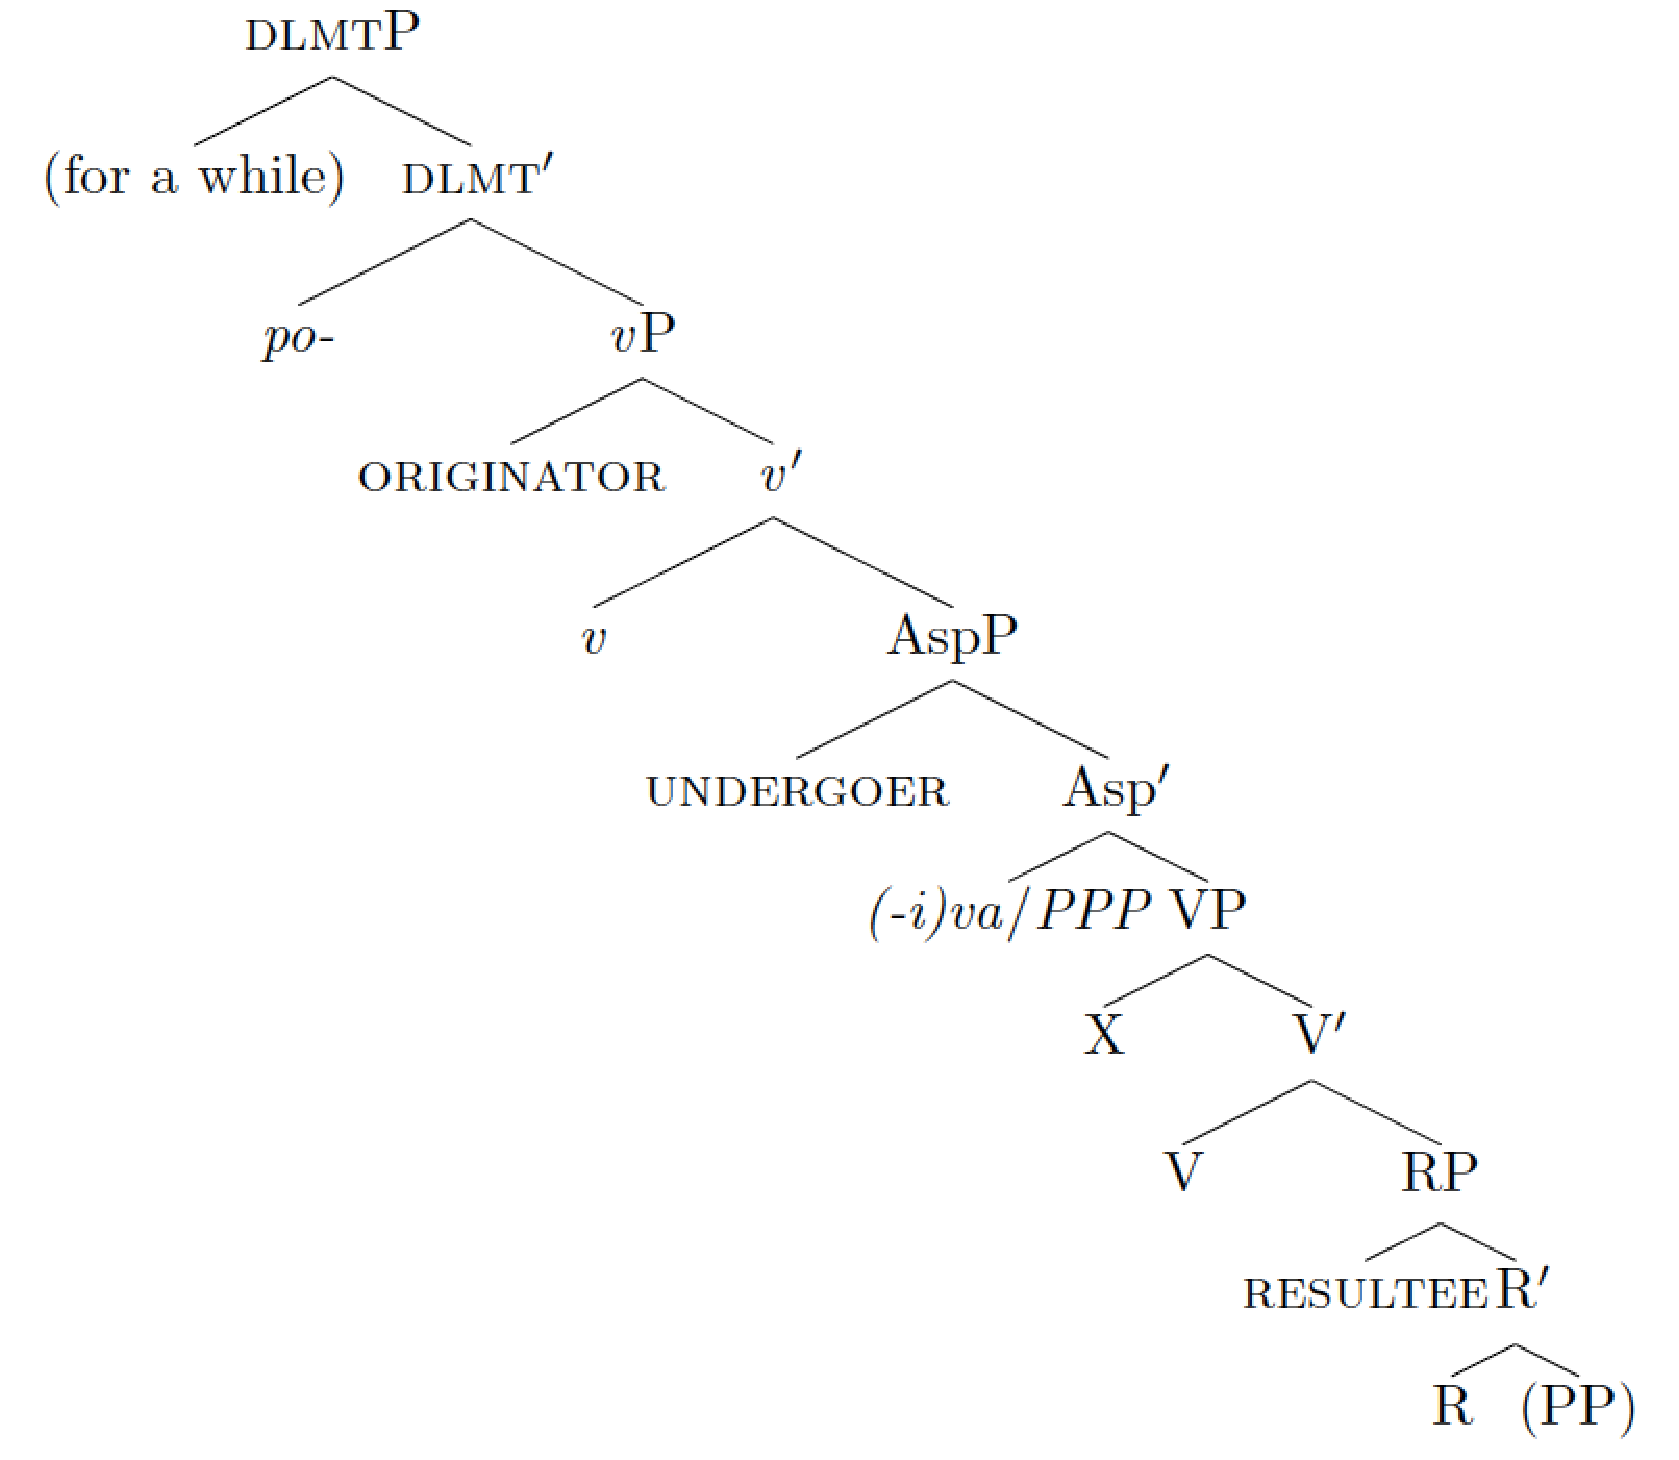
\includegraphics[width=0.8\textwidth]{romanova.pdf}
\caption{\label{fig:romanova} Verbal structure according to \citet[272]{Romanova:04}}
\begin{forest}
[\textsc{dlmt}P
  [(for a while)]
  [\textsc{dlmt}'
    [\textit{po-}]
    [\textit{v}P
      [\textsc{originator}]
      [\textit{v}'
        [\textit{v}]
        [AspP
          [\textsc{undergoer}]
          [Asp'
            [\textit{(-i)va}\slash \textit{PPP}]
            [VP
              [X]
              [V'
                [V]
                [RP
                  [\textsc{resultee}]
                  [R'
                    [R]
                    [(PP)]
                  ]
                ]
              ]
            ]
          ]
        ]
      ]
    ]
  ]
]
\end{forest}
\end{figure}

While \citet{Babko-Malaya:99} and \citet{Schoorlemmer:95} (among others) assume that \isi{superlexical} prefixes form a homogeneous class, \citet{Svenonius:04b} argues that there is a tripartite division among \isi{superlexical} prefixes based on their ability to form secondary imperfectives.

According to \citet{Svenonius:04b}, certain \isi{superlexical} prefixes (\textit{za-} with inceptive meaning, \textit{ot-} with \isi{terminative} meaning, and \textit{pere-} with distributive meaning\footnote{\textit{pere-} has a variety of meanings (e.g. \citealt{Shvedova:82} distinguishes between ten different meanings) including \isi{spatial}, temporal, comparative, iterative, crossing the boundary, distributive, and \isi{excessive} \textit{pere-}. See Section~\ref{subsection:semantics:pere} for more information.}) may be attached higher than the structural position of the \isi{imperfective suffix}, which is \textit{Asp}, the head of \textit{AspP}. Such prefixes disallow the formation of secondary imperfectives (e.g., \textit{za-} in its inceptive use). That is, the \isi{imperfective suffix} cannot be directly attached to an imperfective stem and the result is an invalid structure (see \figref{fig:svenonius}).

There are also mixed cases like \isi{cumulative} \textit{na-}, \isi{excessive} \textit{pere-}, and \isi{attenuative} \textit{po-}. The normal point of attachment of such prefixes, according to \citet[231]{Svenonius:04b}, is outside the scope of the \isi{secondary imperfective}, although under certain exceptional conditions they allow a lower point of attachment.

Svenonius' main generalizations can be stated as follows (see also the summary in \citealt{Svenonius:12}): 

\begin{enumerate}
\item \isi{lexical prefixes} originate inside \textit{v}P;
\item \isi{superlexical} prefixes originate outside \textit{v}P;
\item lexical and \isi{superlexical} prefixes that (according to him) disallow secondary \isi{imperfectivization} are separated by Asp in the \isi{syntactic structure}; 
\item exceptional \isi{superlexical} prefixes are merged (sometimes) outside \textit{v}P, but below the Asp.
\end{enumerate}

\begin{figure}
% % 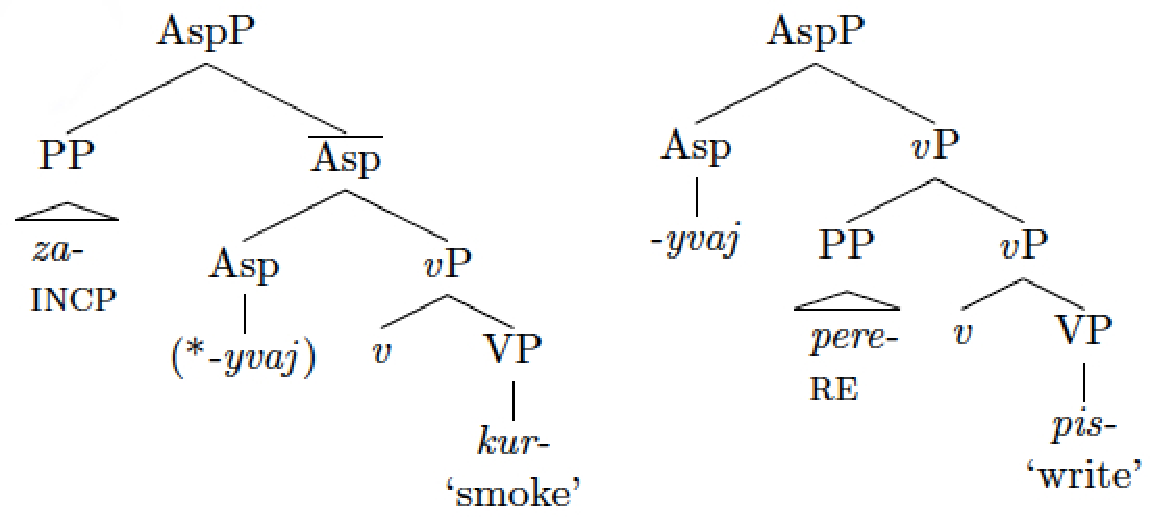
\includegraphics[width=0.8\textwidth]{svenonius.pdf}
\begin{forest}
[AspP
  [PP [\textit{za-}\\\textsc{incp},align=center,roof]]
  [$\overline{\mbox{Asp}}$
    [Asp [(*\textit{-yvaj})]]
    [\textit{v}P
      [\textit{v}]
      [VP
        [\textit{kur-}\\`smoke',align=center]
      ]
    ]
  ]
]
\end{forest}
\begin{forest}
[AspP
  [Asp [-\textit{yvaj}]]
  [\textit{v}P
    [PP [\textit{pere-}\\\textsc{re},align=center,roof]]
    [\textit{v}P
      [\textit{v}]
      [VP [\textit{pis-}\\`write',align=center]]
    ]
  ]
]
\end{forest}
\caption{\label{fig:svenonius}Verbal structure according to \citet[231]{Svenonius:04b}}
\end{figure}

From another study that follows the same tradition, \citealt{Ramchand:04}, the following `bottom-up' order of verbal affixes emerges:

\begin{enumerate}
\item \isi{lexical prefixes};
\item an aspectual head that may contain either the \isi{imperfective suffix} or a \isi{superlexical} prefix;
\item a DP projection for \isi{superlexical} \isi{distributional} prefixes (she cites \textit{pere}- and \textit{po}-). 
\end{enumerate}
While the motivation for this hierarchical order is not entirely clear, it would seem to derive from the following assumptions made by \citet{Ramchand:04}: 
\begin{enumerate}
\item \isi{lexical prefixes} appear low in the \isi{syntactic structure}, due to which a ``presuppositional structure to the aspectual head'' is introduced ``to the effect that it creates a definite rather than an indefinite time moment in Asp'' (p. 349);
\item most \isi{superlexical} prefixes are in Asp and ``impose a specific reference time on the relation between event and temporal anchoring'' (p. 351);
\item a position that \isi{superlexical} prefixes which are \isi{distributional} (\textit{pere}- and distributive \textit{po}-) occupy is higher in the hierarchy than the Asp head (p. 352); such prefixes can be attached directly to the root or to the \isi{secondary imperfective} verb.
\end{enumerate}
The fundamental two-way distinction is of key importance for \citet{Romanova:04}, \citet{Svenonius:04b}, and \citet{Ramchand:04}. Putting it simply, the main idea is that \isi{lexical prefixes} occupy lower positions in the \isi{syntactic tree} than the \isi{superlexical} ones. Though it is possible that there is more than one position for \isi{superlexical} prefixes, all such positions should be higher than the one (unique) position for the \isi{lexical prefixes}. 

Due to this syntactic difference, \isi{superlexical} prefixes are claimed to have the following properties:
\begin{enumerate}
\item they provide a systematic semantic contribution and do not change the lexical meaning of the verb;
\item they are incompatible with secondary \isi{imperfectivization};
\item they do not change the \isi{argument structure} of the verb;
\item they appear to the left of the \isi{lexical prefixes} (if two or more prefixes are stacked). 
\end{enumerate}

Lexical prefixes, on the other hand, are expected to change the lexical meaning of the verb, allow for secondary \isi{imperfectivization}, change the \isi{argument structure} of the verb, and always appear closer to the stem when \isi{prefix stacking} occurs. At the same time two \isi{lexical prefixes} can never stack, as there is a single position where they are allowed. While specific analyses vary a lot, this general idea remains the same. 

The distinction between the lexical and \isi{superlexical} prefixes has received some amount of criticism in the recent literature. For example, \citet{Braginsky:08}, analysing different usages of the prefix \textit{za-}, arrives at the conclusion that ``the contrasts
between \isi{inchoative} and non-\isi{inchoative} prefixes ZA- cannot be accounted for by
simply relating them to different structural positions on the \isi{syntactic tree}'' (p. 224). Let me now analyse in detail properties that are attributed to \isi{superlexical} prefixes and problems that arise when one tries to use the lexical/\isi{superlexical} distinction for analysing \isi{complex verbs} in Russian.

%The assumptions listed above lead to the certain predictions about the grammatical aspect of a given complex verb. First, if a verb contains a prefix and no \isi{imperfective suffix}, it is perfective (see ex.~\ref{pred1}). Second, if a verb contains a \isi{lexical prefix} and the \isi{imperfective suffix}, it is imperfective (see ex.~\ref{pred2}). Finally, if a verb contains a \isi{superlexical} prefix and the \isi{imperfective suffix}, it is perfective (see ex.~\ref{pred3}).

\section{Classification ambiguity}\label{section:classification}
The general problem of the lexical/\isi{superlexical} distinction has been pointed out by \citet[32]{Kagan:book}: many prefixes are not easily classified as either lexical or \isi{superlexical} as they do not have the whole cluster of properties of one of the groups, but rather a mixture. This results in a range of classifications offered by different researchers. Table \ref{table:prefixes} summarizes various proposals in this respect.


\begin{table}
\caption{Superlexical prefix inventory according to different studies\label{table:prefixes}}
\begin{tabular}{lccccccc}
\lsptoprule
prefix &  \rotatebox{90}{\citet{Babko-Malaya:99}} & \rotatebox{90}{\citet{Svenonius:04a}} & \rotatebox{90}{\citet{Svenonius:04b}\footnote{\citet{Svenonius:04b} provides a classification of Russian prefixes from the point of view of the formation of the \isi{secondary imperfective}, but does not state whether the list is exhaustive.}} & \rotatebox{90}{\citet{Ramchand:04}} & \rotatebox{90}{\citet{Romanova:06}} & \rotatebox{90}{\citet{Tatevosov:09}} & \rotatebox{90}{\citet{Svenonius:12}\footnote{\citet{Svenonius:12} marks the list as taken from \cite{Svenonius:04a}, but the lists vary significantly.}}\\
\midrule
\isi{inchoative} \textit{za-} & + & + & + & + & + & + & +\\
\isi{cumulative} \textit{na-} & \textminus & + & + & + & + & + & +\\
saturative \textit{na-} & \textminus & + & \textminus & \textminus & \textminus & \textminus & +\\
\isi{repetitive} \textit{pere-} & \textminus & + & + & \textminus & \textminus & + & +\\
\isi{excessive} \textit{pere-} & \textminus & + & + & \textminus & \textminus & \textminus & +\\
distributive \textit{pere-} & \textminus & \textminus & + & \textminus & + & + & +\\
distributive \textit{po-} & \textminus & + & \textminus & \textminus & + & + & +\\
\isi{delimitative} \textit{po-} & + & + & \textminus & + & + & + & +\\
\isi{attenuative} \textit{po-} & \textminus & + & + &  \textminus & \textminus & \textminus & +\\
\isi{attenuative} \textit{pri-} & \textminus & \textminus & \textminus & \textminus & + & \textminus & \textminus\\
\isi{attenuative} \textit{pod-} & \textminus & \textminus & \textminus & \textminus & + & + & \textminus\\
\isi{terminative} \textit{ot-} & \textminus & + & + & \textminus & + & \textminus & +\\
\isi{perdurative} \textit{pro-} & + & + &  \textminus & \textminus & \textminus & \textminus & +\\
\isi{completive} \textit{iz-} & \textminus & + & + & \textminus & \textminus & \textminus & +\\
\isi{completive} \textit{do-} & \textminus & + &  \textminus & + & \textminus & + & +\\
\lspbottomrule
\end{tabular}
\end{table}

The rows of Table~\ref{table:prefixes} show ten prefixes (\textit{za-, \isi{na-}, \isi{pere-}, \isi{po-}, \isi{pri-}, \isi{pod-}, \isi{ot-}, \isi{pro-}, \isi{iz-}, do-}) together with their interpretations (up to three in case of the prefixes \textit{pere-} and \textit{po-}). The columns of the table represent seven different proposals: \citealt{Babko-Malaya:99}, \citealt{Svenonius:04a}, \citealt{Svenonius:04b}, \citealt{Ramchand:04}, \citealt{Romanova:06}, \citealt{Tatevosov:09}, and \citealt{Svenonius:12}. A plus in the intersection indicates that the prefix of the row (with the fixed interpretation) is listed as \isi{superlexical} in the work that names the column. As \isi{lexical prefixes} are usually not explicitly listed, a minus in the intersection only indicates that the prefix with specific meaning is not listed as \isi{superlexical}.

As is evident from the table, there is only one prefix that is overtly classified as \isi{superlexical} in all the discussed studies: the \isi{inchoative} prefix \textit{za-}. For two more prefixes, \isi{cumulative} \textit{na-} and \isi{delimitative} \textit{po-}, there is almost complete consensus: all but one study describe them as being \isi{superlexical}. Among the remaining prefixes, there is no single prefix listed as \isi{superlexical} in five out of seven discussed works. After this gap comes a group of prefixes that are accepted as \isi{superlexical} in most accounts represented in the table: \isi{repetitive} \textit{pere-}, distributive \textit{pere-}, distributive \textit{po-}, \isi{terminative} \textit{ot-}, and \isi{completive} \textit{do-}. This makes a total of three prefixes in the ``strong'' group and five more in the ``weak'' group. A further seven prefixes are considered \isi{superlexical} only in a couple of studies. Note that there is no pair of works with identical lists of \isi{superlexical} prefixes. 

Such variability in the decisions about which prefix (even under a particular interpretation) falls into one of the two groups (lexical or \isi{superlexical}) clearly shows that this distinction is problematic: the properties that are claimed to be associated with the \isi{superlexical} prefixes do not coincide. I believe that they are not completely independent of each other, but the connection is weaker than is commonly assumed. Let us now discuss different properties attributed to the members of the \isi{superlexical} class of prefixes and see if they are supported by the language data.



\section{Semantics of the derived verb}\label{section:new:compositionality}
The Compositionality of meaning is one of the main characteristics of the \isi{superlexical} prefixes, as shown in the summary provided in Section~\ref{section:properties}. It is important to note, however, that this property is not very valuable if we classify prefixes together with certain fixed interpretations. For instance, if one takes into account only \isi{inchoative} usages of \textit{za-}, then verbs formed with the \isi{inchoative} prefix \textit{za-} will all have the meaning of inception of the activity described by the \isi{derivational base}. All the other \textit{za-}prefixed verbs, even if their semantics is perceived as being close to that of inception, will remain outside the focus set of verbs. This means that when the prefix usages are classified, the property of contributing a compositional meaning is reduced to the productivity of a particular meaning of a given prefix. This said, one has to note that many prefixes that are classified as lexical have systematic transparent contributions: e.g., \isi{spatial} prefixes when combined with motion verbs. Consider, in particular, the \isi{spatial} usage of the prefix \textit{pere-}, `\isi{to cross}'. Whenever this prefix is attached to a directed \isi{motion verb}, it contributes the meaning `\isi{to cross} something in a manner denoted by the \isi{derivational base}', that can also be reformulated as `to perform the motion denoted by the \isi{derivational base} along the path that crosses the landmark'. However, this prefix (and other similar ones) are not considered \isi{superlexical}.

One may reply at this point, that it is not only the systematic semantic contribution, but the absence of change in the lexical meaning, that distinguishes \isi{superlexical} prefixes from lexical ones. Let us consider the verb \textit{proplyt'}$^{\PF}$ `to swim a certain \isi{distance}' and the verb \textit{proplavat'}$^{\PF}$ `to swim for a certain time'. In the first case we are dealing with the \isi{spatial} interpretation prefix \textit{pro-} that is considered to be lexical, while in the second case the same prefix is interpreted temporally and is considered to be \isi{superlexical} by \citet{Babko-Malaya:99}, \citet{Svenonius:04a}, and \citet{Svenonius:12}. Given the semantics of the derived verbs and the possibility of the unified analyses of the prefix \textit{pro-} in these cases \citep{Kagan:book, ZinovaOsswald:paper}, it would be very hard to argue that one of these prefixes affects the lexical meaning of the verb, while the other does not. 

\section{Secondary imperfectivization}\label{section:new:imperfectivization}
Another criterion that is used for establishing the lexical/\isi{superlexical} status of a prefix with a fixed interpretation is the (un)availability of the secondary \isi{imperfectivization}. Basically, superlexically prefixed verbs should not allow secondary \isi{imperfectivization} while lexically prefixed verbs should be easily imperfectivized. Unfortunately, things are not as clear and there are exceptions from this rule in both directions. 

To overcome this difficulty, \citet{Svenonius:04b} and \citet{Tatevosov:07, Tatevosov:09} propose to split \isi{superlexical} prefixes into further groups and to distinguish subclasses of \isi{superlexical} prefixes that allow subsequent \isi{imperfectivization}. Note that in this case the property of used to delimit the classes (nemaly, having potential for further \isi{imperfectivization}), is not derived from other properties of the prefixes.

Furthermore, as is noted by \citet[35]{Kagan:book}, it is not the case that the availability of the \isi{secondary imperfective} verb can be predicted from the knowledge about the last prefix attached to the verb (and its meaning). Distinct stems, when combined with the same prefix (with a fixed interpretation) behave differently: e.g., the verb \textit{naest’sja} `to eat one's fill' is easily imperfectivized and the combination of the verb \textit{nasmotret'sja} `to spend enough time looking at something' with an \isi{imperfective suffix} is weird (example taken from \citealt[35]{Kagan:book}).

Let us examine the \isi{inchoative} prefix \textit{za-} that, according to both \citet[230]{Svenonius:04b} and \citet[116]{Tatevosov:09}, disallows subsequent \isi{imperfectivization}. Consider the verb \textit{kurit'}$^{\IPF}$ `to smoke'. Which can be prefixed with the \isi{inchoative} prefix {\textit{za-}.} The output of \isi{prefixation} is the verb \textit{zakurit'}$^{\PF}$ `to start smoking'. This is a superlexically prefixed verb, according to the common classification, with the most prototypical \isi{superlexical} prefix: the only one which is included in the \isi{superlexical} group in all of the studies I examined. However, this verb can be further imperfectivized. The result of this operation is an imperfective verb \textit{zakurivat'}$^{\IPF}$ `to start/be starting smoking'. As the verb \textit{zakurit'} `to start smoking' denotes a \isi{punctual event}, the natural interpretation of the verb \textit{zakurivat'} `to start/be starting smoking'  is that of a habitual event. Consider example \ref{ex:zakurivat1}. In this sentence the speaker describes his regular activity: after some other event, he always started to smoke and smoked ten cigarettes in a row. 

\exg.\label{ex:zakurivat1}Ja zakurival i kuril desjat' \v{s}tuk, ne vstavaja s mesta, odnu za drugoj.\\
I za.smoke.imp.\glb{pst}.\glb{sg}.\glb{m} and smoke.\glb{pst.sg.m} ten piece.\glb{pl.acc}, not get.up.imp.\glb{cvb}.\glb{pres} from place, one behind other\\
\trans `I started to smoke and smoked ten cigarettes one after another without getting up.'\hbox{}\hfill\hbox{Vasilij Aksenov, \textit{Zv\"{e}zdnyj bilet}}

At the first sight it seems impossible to interpret the resulting imperfective verb progressively. If this were possible, then a possible solution to the problem could be the one by \citet{Ramchand:04}. \citet{Ramchand:04} suggests that \isi{secondary imperfective} forms with a \isi{habitual reading} may be derived by a different imperfectivizing operator from \isi{secondary imperfective} forms with a \isi{progressive reading}. The operator with a \isi{habitual reading} should then be situated higher than the \isi{superlexical} prefix. This proposal does not solve the problem, as it turns out that \isi{progressive interpretation} of the \isi{secondary imperfective} verb containing the \isi{inchoative} \textit{za-} is possible. Out of the blue a native speaker of Russian (without linguistic training) would probably deny the existence of such a reading, but all the speakers I have consulted will accept the sentence \ref{ex:zakurivat2}. The trick here is to find some other event (in this case it is a glance) that takes even less time, and hence is ``more punctual''. Then the event of lighting a cigarette can be viewed as a \isi{progressive one}. We will discuss this issue in more detail in the next chapter.

\exg.\label{ex:zakurivat2}Arkadij Sergeevi\v{c} kak raz zakurival, po\`{e}tomu ne zametil, kak na poslednej fraze Olafson po\v{c}emu-to vorovato strel'nul glazami.\\
Arkadij Sergeevich as time za.smoke.imp\glb{.pst.sg.m}, {that is why} not notice.\glb{pst.sg.m}, as on last phrase Olafson {because of something} thievishly shoot.sem.\glb{pst.sg.m} eye.\glb{pl.inst}\\
\trans `Arkadij Sergeevich was just lighting the cigarette, so he didn't notice Olafson's thievish glance during the last phrase.'\\\hbox{}\hfill\hbox{
Andrej Konstantinov, \textit{Vydum\v{s}\v{c}ik}}

Interestingly, while \citet{Tatevosov:09}, along with \citet{Svenonius:04b}, \citet{Ramchand:04}, and others, postulate the impossibility of subsequent \isi{imperfectivization} of verbs prefixed with \isi{inchoative} \textit{za-} (p.~116), the theory described in the paper does not prohibit it, as \textit{za-} belongs to the group of prefixes that only attach to \isi{imperfective verbs} (more details will follow in Section~\ref{section:Tat09}). This restriction is met in the example above: the verb \textit{kurit'}$^{\IPF}$ `to smoke' is imperfective. It turns out that for \citet{Tatevosov:09} the only group of prefixes that disallow subsequent \isi{imperfectivization} is the group of \isi{left periphery} prefixes which comprises only one prefix: distributive \textit{po-}. This amounts to the fact that one of the main properties of \isi{superlexical} prefixes is attributed to just one prefix which is, moreover, not classified as \isi{superlexical} by some authors.

On the basis of the facts described above I conclude that availability of the \isi{secondary imperfective} form can neither be used for classification purposes nor be reliably predicted from the lexical/\isi{superlexical} status of a given prefix.

\section{Argument structure}\label{section:new:argstructure}
One more property that is said to be associated with \isi{superlexical} prefixes is that they do not change the \isi{argument structure} of the verb (while \isi{lexical prefixes} do). As this criterion is also not unproblematic, \citet[116]{Tatevosov:09}, for example, adopts a milder version of the statement, namely, that \isi{superlexical} prefixes either do not change the \isi{argument structure} of the verb or restrict the possibilities of \isi{argument structure} variation in a predictable way. However, there are exceptions to this property even in the latter formulation. 

The crucial example here is the \isi{cumulative} prefix \textit{na-}, which is considered to be \isi{superlexical} in most studies. However, its attachment changes the \isi{argument structure} of the verb: verbs that are optionally transitive when unprefixed become obligatorily transitive after the attachment of the \isi{cumulative} \textit{na-}, as illustrated by \ref{ex:pref:na1}--\ref{ex:pref:na2}.

\ex.\label{ex:pref:na1}\ag.\label{ex:pref:na1a}Ma\v{s}a s\v{c}itaet$^{\IPF}$ do desjati.\\
Ma\v{s}a count.\glb{pres.3.sg} until ten\\
\trans `Masha can count up to ten.'
\bg.*Ma\v{s}a nas\v{c}itaet$^{\PF}$ do desjati.\label{ex:pref:na1b}\\
Ma\v{s}a na.count.\glb{pres.3.sg} until ten\\

\ex.\label{ex:pref:na2}\ag.*Ma\v{s}a s\v{c}itaet$^{\IPF}$ desjat' konfet.\label{ex:pref:na2a}\\
Ma\v{s}a count.\glb{pres.3.sg} ten.\glb{acc} candies.\glb{gen}\\
\bg.\label{ex:pref:na2b}Ma\v{s}a nas\v{c}itaet$^{\PF}$ desjat' konfet.\\
Ma\v{s}a na.count.\glb{pres.3.sg} ten.\glb{acc} candies.\glb{gen}\\
\trans `Masha's count of candies will be ten.'

This could be still in accordance with the proposal of \citet{Tatevosov:09}, but it turns out that the prefixed verb also provides an additional restriction on the direct object: it must be a measure phrase. The unprefixed verb \textit{s\v{c}itat'}$^{\IPF}$ \mbox{`to count/be counting'} takes as a direct object any plural \isi{accusative noun phrase} (see example \ref{ex:pref:na2a}), whereas the prefixed verb \textit{nas\v{c}itat'}$^{\PF}$ `to count a lot of' does not (see example \ref{ex:pref:na2b}). It requires a measure phrase (example \ref{ex:pref:na3b}), which is not a valid direct object in case of the unprefixed verb \ref{ex:pref:na3a}. 

\ex.\label{ex:pref:na3}\ag.\label{ex:pref:na3a}Ma\v{s}a s\v{c}itaet$^{\IPF}$ konfety.\\
Ma\v{s}a count.\glb{pres.3.sg} candies.\glb{acc}\\
\trans `Masha counts candies.'
\bg.*Ma\v{s}a nas\v{c}itaet$^{\PF}$ konfety.\label{ex:pref:na3b}\\
Ma\v{s}a na.count.\glb{pres.3.sg} candies.\glb{acc}\\

As a result, in all three pairs of examples above involving the verbs \textit{s\v{c}itat'/nas\v{c}itat'} `to count' only one variant (either unprefixed or prefixed) is possible. The unprefixed verb is required in case of an indirect object, as in \ref{ex:pref:na1}, and in case of a direct object that is not a measure phrase, as in \ref{ex:pref:na2}. Only the prefixed verb can be used when the direct object is a measure phrase, as in example \ref{ex:pref:na3}. In fact, there seems to be no construction in which both \textit{s\v{c}itat'} `to count' and \textit{nas\v{c}itat'} `to count a lot of' could be felicitously uttered.

If one considers a pair where the unprefixed verb is obligatorily transitive, as \textit{varit'}$^{\IPF}$ `to cook/be cooking' and \textit{navarit'}$^{\PF}$ `to cook a lot of', it turns out these two verbs require different cases of the object. If the object is an \isi{accusative noun phrase} \ref{ex:pref:navarit:1}, it is only compatible with the unprefixed verb. If it is a \isi{genitive noun phrase}, it is only compatible with the prefixed member of the pair in question, as illustrated by \ref{ex:pref:navarit:2}.

\ex.\label{ex:pref:navarit:1}\ag.\label{ex:varit:1}Ma\v{s}a varit$^{\IPF}$ sup.\\
Ma\v{s}a cook.\glb{pres.3.sg} soup.\glb{acc}\\
\trans `Masha is cooking soup.'
\bg.*Ma\v{s}a navarit$^{\PF}$ sup.\label{ex:navarit1}\\
Ma\v{s}a na.cook.\glb{pres.3.sg} soup.\glb{acc}\\

\ex.\label{ex:pref:navarit:2}\ag.*Ma\v{s}a varit$^{\IPF}$ supa.\label{ex:varit2}\\
Ma\v{s}a cook.\glb{pres.3.sg} soup.\glb{gen}\\
\bg.\label{ex:navarit2}Ma\v{s}a navarit$^{\PF}$ supa.\\
Ma\v{s}a na.cook.\glb{pres.3.sg} soup.\glb{gen}\\
\trans `Masha will cook a lot of soup.'

Interestingly, in the case of the pair \textit{varit'}$^{\IPF}$ `to cook/be cooking' and \textit{navarit'}$^{\PF}$ `to cook a lot of', a measure phrase can be used as a direct object with both verbs, as illustrated by \ref{ex:pref:navarit:3}.

\ex.\label{ex:pref:navarit:3}\ag.\label{ex:varit3}Ma\v{s}a varit$^{\IPF}$ 5 litrov supa ka\v{z}dyj den'.\\
Ma\v{s}a cook.\glb{pres.3.sg} 5 litre.\glb{pl.gen} soup.\glb{gen} every day\\
\trans `Masha cooks five litres of soup every day.'
\bg.\label{ex:navarit3}Ma\v{s}a navarit$^{\PF}$ 5 litrov supa.\\
Ma\v{s}a na.cook.\glb{pres.3.sg} 5 litre.\glb{pl.gen} soup.\glb{gen}\\
\trans `Masha will cook five litres of soup.'

This suffices to show that prefixes that are considered to be \isi{superlexical} can change the \isi{argument structure} of the verb, thereby not only limiting the existing options for the \isi{derivational base} verb, but also adding new ones.

Now we consider the other direction: if the attachment of a \isi{superlexical} prefix can lead to changes in the \isi{argument structure} of the \isi{derivational base} verb, we can try to reformulate the property. An alternative formulation would be to postulate that if a \isi{lexical prefix} is attached to a verb, argument structures of the source and the derived verb will be distinct. This, however, does not work either. As an example, consider the pair of verbs \textit{delat'/sdelat'} `to do'. Both verbs are obligatorily transitive. Illustrations of this fact are provided in \ref{ex:delat} and \ref{ex:sdelat}.

\ex.\label{ex:delat}\ag.Petja delaet$^{\IPF}$ doma\v{s}nee zadanie.\\
Petja do.\glb{pres.3.sg} home.\glb{sg.acc} assignment.\glb{sg.acc}\\
\trans `Petja is doing his homework.'
\bg.*Petja delaet$^{\IPF}$.\\
Petja do.\glb{pres.3.sg}\\

\ex.\label{ex:sdelat}\ag.Petja sdelaet$^{\PF}$ doma\v{s}nee zadanie.\\
Petja s.do.\glb{pres.3.sg} home.\glb{sg.acc} assignment.\glb{sg.acc}\\
\trans `Petja will do his homework.'
\bg.*Petja sdelaet$^{\PF}$.\\
Petja s.do.\glb{pres.3.sg}\\


As one may object that the prefix \textit{s-} in \textit{sdelat'} `to do' is what some researchers call an ``\isi{empty prefix}'' (a prefix that changes the aspect, but does not lead to a clear change of the lexical meaning, \textit{\v{c}istovidovaja pristavka} in the Russian tradition), let me provide another example where the prefix is clearly not an ``empty'' one, but, according to those who use the lexical/\isi{superlexical} distinction, a lexical one.  Consider the following three verbs: \textit{nesti}$^{\IPF}$ `to carry', \textit{prinesti}$^{\PF}$ `to carry to some destination',  and \textit{otnesti}$^{\PF}$ `to carry away from some location'. All three verbs have the same \isi{argument structure}: they are obligatorily transitive (see examples \ref{ex:nesti}--\ref{ex:otnesti}).

\ex.\label{ex:nesti}\ag.Petja nes\"{e}t$^{\IPF}$ korobku v podval.\\
Petja carry.\glb{pres.3.sg} box.\glb{sg.acc} in cellar.\glb{sg.prp}\\
\trans `Petja is carrying the box to the cellar.'
\bg.*Petja nes\"{e}t$^{\IPF}$ v podval.\\
Petja carry.\glb{pres.3.sg} in cellar.\glb{sg.prp}\\

\ex.\label{ex:prinesti}\ag.Petja prines\"{e}t$^{\PF}$ korobku v podval.\\
Petja pri.carry.\glb{pres.3.sg} box.\glb{sg.acc} in cellar.\glb{sg.prp}\\
\trans `Petja will carry the box to the cellar.'
\bg.*Petja prines\"{e}t$^{\PF}$ v podval.\\
Petja pri.carry.\glb{pres.3.sg} in cellar.\glb{sg.prp}\\

\ex.\label{ex:otnesti}\ag.Petja otnes\"{e}t$^{\PF}$ korobku v podval.\\
Petja ot.carry.\glb{pres.3.sg} box.\glb{sg.acc} in cellar.\glb{sg.prp}\\
\trans `Petja will carry the box to the cellar.'
\bg.*Petja otnes\"{e}t$^{\PF}$ v podval.\\
Petja ot.carry.\glb{pres.3.sg} in cellar.\glb{sg.prp}\\

This clearly shows that knowing the lexical or \isi{superlexical} status of a prefix is not sufficient to predict whether its attachment will change the \isi{argument structure} of the \isi{derivational base} verb.
\section{Position in the stem}\label{section:new:position}
The least problematic property of \isi{superlexical} prefixes is that they always appear to the left of the \isi{lexical prefixes} if two or more prefixes are stacked. When formulated this way, the property holds. However, a stronger version of this statement is used in the literature, either explicitly \citep{Svenonius:04b} or implicitly \citep{Tatevosov:09}: because there is only one syntactic position a \isi{lexical prefix} can appear in, it is assumed that \isi{lexical prefixes} can only appear directly to the left of the verbal root and cannot be stacked. For example, \citet[206]{Svenonius:04b} writes: ``\isi{lexical prefixes} are unique in each VP, as their structural position is unique -- a single V cannot have more than one \isi{resultative} complement.''


This, however, does not hold. Consider, for example, the verb \textit{razukrasit'} `to decorate' and the verb \textit{razuznat'} `to find out'. Each of these verbs contains two prefixes, \textit{raz-} and \textit{u-}, both of which are lexical: if one consults Table~\ref{table:prefixes} again, neither of the prefixes is classified as \isi{superlexical} in any of the papers discussed. The derivation chains for the verbs are constructed using the criteria formulated in Chapter~\ref{Chapter2} and provided in \ref{schema:razukrasit'} and \ref{schema:razuznat'}.

\ex.\ag.\label{schema:razukrasit'}krasit'$^{\IPF}$ {$\rightarrow$} ukrasit'$^{\PF}$ {$\rightarrow$} razukrasit'$^{\PF}$\\
{to paint} {} {to embellish} {} {to decorate}\\
\bg.\label{schema:razuznat'}znat'$^{\IPF}$ {$\rightarrow$} uznat'$^{\PF}$ {$\rightarrow$} razuznat'$^{\PF}$\\
{to know} {} {to learn} {} {to find out}\\
\bg.*lo\v{z}it'$^{\IPF}$ {$\rightarrow$} polo\v{z}it'$^{\PF}$ {$\rightarrow$} raspolo\v{z}it'$^{\PF}$\label{schema:raspolozit'}\\
{to put} {} {to put} {} {to position}\\

A similar case is presented in \ref{schema:raspolozit'}
with the difference that in contemporary literary Russian the unprefixed verb \textit{*lo\v{z}it'}$^{\IPF}$ does not exist (it exists in the colloquial language and in dialects). 

From observing these three examples one may, for the sake of saving the hypothesis of a single position for \isi{lexical prefixes}, hypothesize that the prefix \mbox{\textit{\isi{raz-}/ras-}} is a \isi{superlexical} one. The problem with this hypothesis is that if one believes that the contributions of lexical and \isi{superlexical} prefixes have particular characteristics, then the semantics of this prefix patterns with the semantics of \isi{lexical prefixes}: a thorough study was performed by \citet{JandaNesset:10}, who list eleven subclasses for the meaning that is contributed by the prefix \textit{raz-}, and only one of them (Complex Act Perfective in their terminology) is characteristic of the typical contribution of a \isi{superlexical} prefix.

%\iffalse

\section{Subclasses of superlexical prefixes}\label{section:subclasses}
So far we have observed that the binary distinction between lexical and \isi{superlexical} prefixes is not sufficient to predict the existence and properties of verbs containing certain sets of affixes. As at least some of the problems mentioned above were noticed by the researchers working on Russian \isi{prefixation}, several refinements of the original distinction have been proposed in the literature. In further developments of Russian \isi{prefixation} theories we see a shift of focus from the bipartite distinction to the split of the whole class of prefixes into more than two groups: \citet{Tatevosov:07} proposes a \isi{three-way classification} of verbal prefixes and \citet{Tatevosov:09} splits the class of \isi{superlexical} prefixes into three subclasses.

\subsection{Intermediate prefixes}
\cite{Tatevosov:07} introduces a class of \isi{intermediate prefixes} that is supposed to accommodate prefixes which do not fit nicely into either the lexical or the \isi{superlexical} category. This class comprises the \isi{completive} prefix \textit{do-} and the \isi{repetitive} prefix \textit{pere-}. \citet{Tatevosov:07} proposes that these prefixes are structurally higher than \isi{lexical prefixes}, but lower than \isi{superlexical} prefixes and the \isi{secondary imperfective}. 

This division is motivated by examples like \ref{ex:naperf} and \ref{ex:pereimp}. For the analysis that assumes the two-way classification of prefixes, the verbs \ref{ex:naperf} and \ref{ex:pereimp} have identical \isi{internal} structure: a \isi{superlexical} prefix, a \isi{lexical prefix}, a stem, and the \isi{imperfective suffix}. Nevertheless, these verbs are assigned different aspects: the verb \textit{nazapisyvat'} `to write down a lot' is perfective while the verb \textit{perezapisyvat'} `to be rewriting/to rewrite' is imperfective. For \citet{Tatevosov:07}, there is a structural difference between the two verbs, because \textit{pere}- is classified as an intermediate prefix and is positioned between \isi{lexical prefixes} and the \isi{imperfective suffix}. As a result, the verb in \ref{ex:pereimp} is assigned the imperfective aspect. At the same time, \textit{na}- remains a \isi{superlexical} prefix and thus the verb \textit{nazapisyvat'} `to write down a lot' is assigned the perfective aspect.
\ex.\ag.\label{ex:naperf}nazapisyvat'$^{\PF}$\\
na.za.write.imp.\glb{inf}\\
`to write down a lot'
\bg.\label{ex:pereimp}perezapisyvat'$^{\IPF}$\\
pere.za.write.imp.\glb{inf}\\
`to be rewriting/to rewrite'

However, \cite{Kagan:book} shows that the introduction of \isi{intermediate prefixes} does not solve the problem of predicting the aspect of a given verb on the basis of information about the affixes it is formed with: she provides examples where verbs prefixed with the \isi{attenuative} prefix \textit{pod-} allow the subsequent formation of the \isi{secondary imperfective} \citep[35, ex.~\ref{ex:pod} here]{Kagan:book}

\ex.\label{ex:pod}\ag.pod-taj-a-t' - pod-taj-iva-t'\\
pod.melt.\glb{inf} - pod.melt.imp.\glb{inf}\\
melt slightly$^{\PF}$ - melt slightly$^{\IPF}$
\bg.\label{ex:podustavat'}pod-u-st-a-t' - pod-u-sta-va-t'\\
pod.get.tired.\glb{inf} - pod.get.tired.imp.\glb{inf}\\
get tired slightly$^{\PF}$ - get tired slightly$^{\IPF}$
\bg.\label{ex:podzarabatyvat'}pod-za-rabot-a-t' - pod-za-rabat-yva-t'\\
pod.earn.\glb{inf} - pod.earn.imp.\glb{inf}\\
earn some money$^{\PF}$ - earn some money$^{\IPF}$

\cite{Kagan:book} marks imperfective forms in \ref{ex:podustavat'} and \ref{ex:podzarabatyvat'} with \textit{??} and \textit{*} respectively, as out of \isi{context} these forms sound weird to a native Russian speaker. However, if one needs to express the meaning `earn a small amount of money from time to time' the best way to do it is to use the verb \textit{podzarabatyvat'}. As soon as it is put in the \isi{context}, as in \ref{ex:podzarabatyvat'live}, this verb starts to sound natural and may be marked with a question, but is definitely not ungrammatical. I hypothesize that the oddness of the \isi{secondary imperfective} here can be of the same sort as the oddness of multiply prefixed verbs: it is almost impossible to process such verbs without a \isi{context} and thus they are perceived as unnatural when given in isolation, but become fine in an appropriate setting.

\exg.\label{ex:podzarabatyvat'live}Delaete xoro\v{s}ie fotosnimki? U vas est' vozmo\v{z}nost' podzarabatyvat' na \`{e}tom!\\
make good photos near you have possibility pod.za.earn.imp.\glb{inf} on this\\
\trans `Do you take good photos? You have the chance to earn some money from it!'~~\hbox{}\hfill\hbox{\url{http://smolgorforum.ru}}

This suffices to show that the classification provided by \citet{Tatevosov:07} does not allow one to reliably predict the aspect of the complex verb, despite the fact that this task can be viewed as the driving force of the proposed approach. 

\subsection{A three-way distinction}\label{section:Tat09}
%\label{section:selection}
A more elaborate classification is proposed in \citealt{Tatevosov:09}, which is mainly dedicated to the problem of \isi{prefix stacking}. However, in order to account for the relevant stacking constraints, the proposal amounts to a list of postulations about the position of prefixes in the \isi{syntactic tree}. \citet{Tatevosov:09} abandons the previous tripartite distinction among all the prefixes, proposed in \citet{Tatevosov:07}, and instead argues for a classical bipartite division into lexical and \isi{superlexical} prefixes, enriching it with a \isi{three-way classification} of the \isi{superlexical} prefixes in order to account for the relevant facts: \isi{left periphery} prefixes, \isi{selectionally limited prefixes}, and \isi{positionally limited prefixes}.

The group of \isi{left periphery} prefixes comprises only one prefix: distributive \textit{po}- (as in \textit{pobrosat'} `to throw all of'). It occupies the \isi{left periphery} of the verbal structure.

Selectionally limited prefixes can be added only to a formally imperfective verb. The group includes the \isi{delimitative} prefix \textit{po}- (\textit{posidet'} `to sit for some time'), the \isi{cumulative} prefix \textit{na}- (\textit{navarit'} `to cook a considerable amount of something'), the distributive prefix \textit{pere}- (\textit{perelovit' X} `to catch all of X'), and the \isi{inchoative} prefix \textit{za}- (\textit{zabegat'} `to start running around').

The last group of \isi{positionally limited prefixes} contains the \isi{completive} prefix \textit{do}- (\textit{dodelat'} `to finish doing'), the \isi{repetitive} prefix \textit{pere}- (\textit{perepisat'} `to rewrite'), and the \isi{attenuative} prefix \textit{pod}- (\textit{podustat'} `to become a little bit tired'). These prefixes, according to \citet{Tatevosov:09}, can be added only before\footnote{The attachment of one affix \textit{before} the other is understood in terms of the derivation chain: the first affix is attached at the earlier step of the derivation. This amount to a lower attachment site in terms of the tree structure.} the \isi{secondary imperfective} suffix -\textit{yva-/-iva}- and end up in the same structural position as \isi{intermediate prefixes} in \citet{Tatevosov:07}, the group being extended by one prefix.
	
The net advantage of \citet{Tatevosov:09} over \citet{Tatevosov:07} seems to be that only the former can correctly predict the existence of the derived verbs in \ref{ex:pod} and motivate the difference between \ref{ex:ponaza} and \ref{ex:napoza}. The drawback caused by the need to structurally distinguish cases like \ref{ex:ponaza} and \ref{ex:napoza} is the stipulation that distributive prefix \textit{po-} forms a singleton group. On \citeauthor{Tatevosov:09}'s (2009) account, distributive \textit{po}- must be situated on the \isi{left periphery} of the verb, thus there can be no derivation for \ref{ex:napoza}.
\ex.\ag.\label{ex:ponaza}ponazapisyvat'\\
po.na.za.write.imp.\glb{inf}\\
\trans `to write down all of X one after another'
\bg.\label{ex:napoza}*napozapisyvat'\\
na.po.za.write.imp.\glb{inf}\\

In general, the theory proposed by \citet{Tatevosov:09} seems to account nicely for many cases of multiple \isi{prefixation} of Russian verbs. Let us for the moment set aside the problem of \isi{biaspectual verbs} described in Section~\ref{section:new:biaspectual} as well as the problem of a singleton group, mentioned above, and concentrate on one of the central predictions of the theory: \isi{selectionally limited prefixes} can be attached only to formally \isi{imperfective verbs}.

It turns out that it is possible to find examples where prefixes that are supposed to belong to the selectionally-limited group are attached to formally \isi{perfective verbs}, which contradicts the proposed theory of \isi{prefixation}. We will look in turn at the prefixes \textit{po-} (\isi{delimitative}), \textit{pere-} (distributive), and \textit{na-} (\isi{cumulative}). 

\subsubsection{Delimitative \textit{po-}}
First let us consider examples where the \isi{delimitative} prefix \textit{po-} can indeed only be added to an imperfective verb. In case of an \isi{aspectual pair} where both verbs are unprefixed (as, for example, \textit{re\v{s}it'}$^{\PF}$\slash\textit{re\v{s}at'}$^{\IPF}$ `to solve') the prefix \textit{po-} can only be combined with the imperfective member of the pair (in this case \textit{re\v{s}at'}$^{\IPF}$ `to solve/be solving'), as illustrated by example \ref{ex:po:Tat1} (example (62b) in \citealt[121]{Tatevosov:09}). If the paired verbs both contain a prefix, as \textit{zapisat'}$^{\PF}$\slash\textit{zapisyvat'}$^{\IPF}$ `to write down/record', the \isi{delimitative} prefix \textit{po-} is normally attached to the imperfective verb (in this case \textit{zapisyvat'}$^{\IPF}$ `to write down/be writing down'), as illustrated by example \ref{ex:po:Tat2} (example (63b) in \citealt[121]{Tatevosov:09}).

\ex.\label{ex:po:Tat}\ag.\label{ex:po:Tat1}Posidim, *pore\v{s}im (\textsuperscript{\JudgeOK}pore\v{s}aem$^{\PF}$) voprosy, s pacanami poznakomi\v{s}sja, \v{c}toby dorogu slu\v{c}ajno ne perebegat'.\\
po.sit.\glb{pres.1.pl}, *po.solve.\glb{pres.1.pl} (\textsuperscript{\JudgeOK}po.solve.imp.\glb{pres.1.pl}) question.\glb{pl.acc}, with boy.\glb{pl.inst} po.meet.\glb{pres.1.pl}.refl, that road.\glb{sg.acc} {by chance} not pere.run.\glb{inf}\\
\trans `We will sit a bit, solve some issues, you will get to know the boys so that you won't accidentally cross their way.'\\\hbox{}\hfill\hbox{Gennadij Pra\v{s}kevi\v{c}, Aleksandr Bogdan, \textit{\v{C}elovek ``\v{C}''}}\\\hbox{}\hfill\hbox{(62b) in \citet{Tatevosov:09}}
\bg.\label{ex:po:Tat2}Po\`{e}tomu zapustil programmu, zapisyvaju\v{s}\v{c}uju dejstvija na \`{e}krane, otkryl PSP, i nemnogo $^\#$po-zapisal (\textsuperscript{\JudgeOK}po-zapisyval$^{\PF}$), \v{c}to i kak.\\
{because of it} za.let.\glb{pst.sg.m} program.\glb{sg.acc}, za.write.\glb{part.act.pres.sg.f.acc} action.\glb{pl.acc} on screen.\glb{sg.prep}, open.\glb{pst.sg.m} PSP, and {a bit} $^\#$po.write.\glb{pst.sg.m} (\textsuperscript{\JudgeOK}po.write.imp\glb{pst.sg.m}), what and how\\
\trans `For this reason I ran the program that records the actions on the screen and recorded for some time, what was happening and how.'\\\hbox{}\hfill\hbox{=(63b) in \citet{Tatevosov:09}, \url{nova-forum.com}}

Now let me providesome examples where the \isi{delimitative} prefix \textit{po-} is attached to a formally perfective verb. In the first example, \ref{ex:popriotkryl}, we are dealing with a selectionally limited prefix \textit{po-} that is attached to the perfective verb \textit{priotkryt'}$^{\PF}$ `to open slightly.' The \isi{derivational base} verb already contains the \isi{attenuative} prefix \textit{pri-}, so the \isi{delimitative} prefix \textit{po-} plays a role of an intensifier of the low degree property. 
\exg. \label{ex:popriotkryl}A na e\v{s}elone on nemno\v{z}ko \v{c}ut' popriotkryl oko\v{s}ko.\\
But at {flight level} he {a little bit} {slightly} po.pri.open.\glb{pst.sg.m} window.\glb{sg.acc}\\
\trans `And at flight level he opened the window just a little bit.'\\\hbox{}\hfill\hbox{\url{www.rsdn.ru/forum}}

Example \ref{ex:popriotkryl} contains a verb that is the result of attaching the \isi{delimitative} prefix \textit{po-} to the perfective verb \textit{priotkryt'}$^{\PF}$ `to open slightly'. We can try to attach the same prefix to the paired imperfective verb \textit{priotkryvat'}$^{\IPF}$ `to open/be opening slightly'. It turns out that the verb that contains all the morphemes of the verb \textit{priotkryvat'}$^{\IPF}$ `to open/be opening slightly' plus the prefix \textit{po-} is the verb \textit{popriotkryvat'} `to slightly open some of X'. This verb cannot be substituted for the verb \textit{popriotkryt'}$^{\PF}$ `to open slightly' in \ref{ex:popriotkryl} without changing the meaning of the sentence: \ref{ex:popriotkryval:mod} means that every time the described person flies on the plane, he opens the window. Moreover, the verb \textit{popriotkryvat'} `to slightly open some of X' is imperfective, unlike the verb \textit{pozapisyvat'} `to record for a while' in example \ref{ex:po:Tat2}.

\exg. \label{ex:popriotkryval:mod}A na e\v{s}elone on nemno\v{z}ko \v{c}ut' popriotkryval$^{\IPF}$ oko\v{s}ko.\\
but at {flight level} he {a little bit} {slightly} po.pri.open.imp.\glb{pst.sg.m} window.\glb{sg.acc}\\
\trans `And at flight level he used to open the window just a little bit.'

Another example is provided in \ref{ex:popod-}. Again, the \isi{delimitative} prefix \textit{po-} seems to be redundant as it contributes the \isi{delimitative} semantics that is already present in the semantic representation of the \isi{derivational base} (just because this is the condition under which it can be attached).

\exg.\label{ex:popod-}Za sorok let despotizma mozgi popodsoxli.\\
after forty year.\glb{pl.gen} despotism brain.\glb{nom} po.pod.dry.\glb{pst.pl}\\
\trans `During forty years of despotism his brain kind of dried up a bit.'\\\hbox{}\hfill\hbox{\url{http://otvet.mail.ru/question/65535779}}

Like example \ref{ex:popriotkryl}, in example \ref{ex:popod-} it is impossible to substitute the verb \textit{popodsoxli}$^{\PF}$ `dried a bit' with the verb \textit{popodsyxali}$^{\PF}$ `all of them dried a bit' which is derived with an additional step of \isi{imperfectivization} in between the two prefixations. The modified sentence in \ref{ex:popod-imp} can only be interpreted as the `brain drying' within a group of people, not only with one person.  

\exg.\label{ex:popod-imp}Za sorok let despotizma mozgi popodsyxali.\\
after forty year.\glb{pl.gen} despotism brain.\glb{nom} po.pod.dry.imp.\glb{pst.pl}\\
\trans `During forty years of despotism their brains kind of dried up.'

The conclusion that can be drawn from the examples above is that although in general the \isi{delimitative} prefix \textit{po-} attaches to \isi{imperfective verbs}, there are some exceptions to this rule. It also turns out that when we encounter an example of a perfective verb prefixed with the \isi{delimitative} \textit{po-}, it is not possible to substitute this verb with the result of the \isi{prefixation} with \textit{po-} of the paired imperfective verb without a change in the semantics of the sentence. This means that in cases like \ref{ex:popriotkryl} and \ref{ex:popod-} the perfective verb prefixed with \textit{po-} cannot be regarded as a ``variant'' of the verb that obeys the selectional restriction.
 
\subsubsection{Distributive \textit{pere-}}
Another prefix that is categorized as selectionally limited by \citet{Tatevosov:09} is the distributive prefix \textit{pere-}. It turns out that there are examples where this prefix is attached to a formally perfective verb, although on the intuitive level the attachment of a distributive \textit{pere-} to a perfective verb seems to be more an exception than a rule. Consider the verb \textit{prosit'}$^{\IPF}$ `to ask'. It can be prefixed with a \isi{lexical prefix} \textit{o-}. The result of this \isi{prefixation} is a perfective verb \textit{oprosit'}$^{\PF}$ `to interview'. This verb can be prefixed with the prefix \textit{pere-}, producing the verb \textit{pereoprosit'}$^{\PF}$ as the output of the \isi{prefixation}. The question now is, which meaning does \textit{pere-} have in this verb? According to \citet{Tatevosov:09}, it could be only iterative \textit{pere-}. This meaning is indeed attested, as illustrated by the example in \ref{ex:pereoprosil:iter}, where \textit{pereoprosil} means `interviewed again'.
\exg.\label{ex:pereoprosil:iter}Sledovateli Genprokuratury zanovo pereoprosili u\v{c}itelej i odnoklassnikov Jakova.\\
investigator.\glb{pl.nom} General.Prosecution.\glb{gen} anew pere.o.ask.\glb{pst.pl} teacher.\glb{pl.acc} and classmate.\glb{pl.acc} Jakov.\glb{gen}\\
\trans `Investigators from the General Prosecution interviewed the teachers and the classmates of Jakov again.'\hbox{}\hfill\hbox{\url{http://cripo.com.ua}}

However, the distributive meaning of \textit{pere-} is also available: sentence \ref{ex:pereoprosil:distr} is true if the speaker posted on each forum and asked every mechanic only once.

\exg.\label{ex:pereoprosil:distr}Perepostil na vse alfaforumy, pereoprosil vsex znakomyx avtoslesarej.\\ 
pere.post.\glb{pst.sg.m} on all {alfa.forums}, pere.ask.\glb{pst.sg.m} all.\glb{acc} known mechanic.\glb{pl.gen}\\
\trans `I posted it on all the major forums and asked all mechanics I know.'\\\hbox{}\hfill\hbox{\url{http://fiat-club.org.ua}}

Let us now consider the case of attaching the prefix \textit{pere-} to an imperfective verb. The verb \textit{oprosit'}$^{\PF}$ `to interview' can be imperfectivized, providing a paired verb \textit{opra\v{s}ivat'}$^{\IPF}$ `to interview/be interviewing'. If this verb is prefixed with \textit{pere-}, the result of the \isi{prefixation} is the verb \textit{pereopra\v{s}ivat'}$^{\PF}$ `to interview all of'. An example of the usage of this verb, found on the internet, is provided in \ref{ex:pereoprashival}. Like in \ref{ex:pereoprosil:distr}, it is clear from the \isi{context} that each of the scientists was asked separately and only once. Normally in a similar \isi{context} one would use the verb \textit{perespra\v{s}ivat'}$^{\PF}$ `to ask all of', as \textit{spra\v{s}ivat'}$^{\PF}$ `to ask' refers to an individual question and the prefix \textit{pere-} then provides iteration over the referents. On the other hand, the verb \textit{opra\v{s}ivat'}$^{\PF}$ `to interview' already encodes iteration of the questions, so after the attachment of the distibutive \textit{pere-} the resulting verb denotes an event that contains a double iteration: every respondent is asked every question. In case of \ref{ex:pereoprashival}, the speaker (or his hero in the computer game the forum is about) asked any other characters of the ``scientist'' type all the possible questions (limited by the game design).

\exg.\label{ex:pereoprashival}Pereopra\v{s}ival vsex u\v{c}\"{e}nyx, nikto ne da\"{e}t kvest na oazis...\\
pere.o.ask.imp.\glb{pst.sg.m} all.\glb{acc} scientist.\glb{pl.gen}, nobody not give.\glb{pres.3.sg} quest on oasis.\glb{sg.acc}\\
\trans `I've talked (asked all the questions) to all the scientists, none of them gave me the oasis quest.'\hbox{}\hfill\hbox{\url{http://antistarforce.com/forum}}

\subsubsection{Cumulative \textit{na-}}
An interesting discussion can be found in \citet{Tatevosov:13a}. It concerns the possibility of attaching the \isi{cumulative} prefix \textit{na-} to a perfective verb. Citing \citet{Zaliznjak:03}, \citet{Tatevosov:13a} concludes that there is a closed list of verbs consisting of a perfective stem prefixed with the \isi{cumulative} \textit{na-} that are accepted by all Russian native speakers. \citet{Tatevosov:13a} mentions, for instance, the verbs \textit{nakupit'}$^{\PF}$ `to buy a lot of something' and \textit{napustit'}$^{\PF}$ `to fill something with a lot of something'. 

\citeauthor{Tatevosov:13a} also writes, however, about another, much larger group of verbs that are formed according to this pattern. This group, according to him, includes such verbs as \textit{napridumat'}$^{\PF}$ `to come up with a lot of something', \textit{narasskazat'}$^{\PF}$ `to tell a lot of something', and \textit{naso\v{c}init'}$^{\PF}$ `to write/compose a lot of something'. Consider example \ref{ex:nazapostil}, taken from the internet. Here we see two verbs formed by \isi{prefixation} of a perfective verb with the \isi{cumulative} prefix \textit{na-}: \textit{naotkryt'} `to open a lot of X' and \textit{nazapostit'} `to write and publish a lot of posts.'
 
\exg.\label{ex:nazapostil}I naotkryl i nazapostil mnogo tem.\\
and na.open.\glb{pst.sg.m} and {na.write.\glb{pst.sg.m}} {many} {topics}\\
\trans `And started a lot of posts and wrote about a lot of topics.'\\\hbox{}\hfill\hbox{\url{http://forum.hayastan.com}}

\citet{Tatevosov:13a} claims that there is quite a large group of people who speak a dialect of Russian where the \isi{cumulative} prefix \textit{na-} lacks any \isi{syntactic restrictions} and can be freely attached to \isi{perfective verbs}. Two problems arise with this claim.

First, the distinction between the ``major'', more restrictive dialect and the dialects that allow freer attachment of the \isi{cumulative} \textit{na-} seems to be not so clearcut. For example, for me as a native speaker of Russian there is a difference in the acceptability of the two verbs in \ref{ex:nazapostil}: the verb \textit{naotkryt'} `to open a lot of X' seems to be considerably less acceptable than the verb \textit{nazapostit'} `to post a lot'. This may be due to the fact that the verb \textit{naotkryt'} `to open a lot of X' can be replaced by another verb in which the \isi{cumulative} \textit{na-} is attached to the imperfective stem: \textit{naotkryvat'}$^{\PF}$ `to open a lot of X' derived from \textit{otkryvat'}$^{\IPF}$ `to open/be opening'. The verb \textit{nazapostit'} `to post a lot', however, lacks a similar paired verb: if I try to form a \isi{secondary imperfective} from the verb \textit{zapostit'} `to post', none of the resulting forms sounds acceptable, possibly for phonological reasons: $^?$\textit{zapostivat'}, $^?$\textit{zapos\v{c}ivat'}, $^?$\textit{zapo\v{s}\v{c}ivat'}, $^?$\textit{zapo\v{s}\v{c}\v{s}\v{c}ivat'}. Interestingly, all of these forms are attested on the internet, as evidenced by the examples in \ref{ex:zapostivat} (with the third variant, \textit{zapo\v{s}\v{c}ivat'}, being the most frequent).

\ex.\label{ex:zapostivat}\ag.Ix teksty ja zapostival na na\v{s} fakul'tetskij forum.\\
they.\glb{gen} text.\glb{pl.acc} I za.post.imp.\glb{pst.sg.m} on our department.\glb{sg.acc.m} forum.\glb{sg.acc}\\
\trans `Their texts I've posted on the forum of our department.'\\\hbox{}\hfill\hbox{\url{hgr.livejournal.com}}
\bg.Tak ponevole bude\v{s} prosit' razre\v{s}enija, esli u\v{z}e raz zapos\v{c}ival, tak pot\"{e}rli.\\
so unwillingly will.\glb{2.sg} ask.\glb{inf} permission.\glb{sg.acc}, if already once za.post.imp.\glb{pst.sg.m}, so po.rub.\glb{pst.pl}\\
\trans `If you already posted something once and it was erased, you inevitably start to ask for permission.'\hbox{}\hfill\hbox{\url{www.forumavia.ru}}
\bg.Davnen'ko ja ni\v{c}ego ne zapo\v{s}\v{c}ival, no dejstvitel'no pisat' ne o \v{c}em.\\
{quite a while} I nothing not za.post.imp.\glb{pst.sg.m}, but really write.\glb{inf} not about that.\glb{prp}\\
\trans `I haven't posted anything for quite a while, but I really have nothing to write about.'\hbox{}\hfill\hbox{\url{www.drive2.ru}}
\bg.Reporta\v{z} 1 kanala RF o poxoronax desantnika ja u\v{z}e zapo\v{s}\v{c}\v{s}\v{c}ival.\\
reportage.\glb{sg.acc} 1 channel {Russian Federation} about funeral.\glb{prp} paratrooper.\glb{sg.gen} I already za.post.imp.\glb{pst.sg.m}\\
\trans `I've already posted the documentary of the first federal channel about the funeral of a paratrooper.'\hbox{}\hfill\hbox{\url{waronline.org}}

The fact that all the possible variants of forming a \isi{secondary imperfective} from the verb \textit{zapostit'} `to post' are attested on the internet indicates that neither of these variants is perfect and acceptable by all speakers.

Now let us explore another problem that arises if we postulate the absence of any restrictions on the attachment of the prefix \textit{na-} for some dialects of Russian, as \citet{Tatevosov:13a} does. The speakers of such a dialect should be able, for example, to derive the verb \textit{naotkryt'}$^{\PF}$ `to open a lot of X' and then imperfectivize it by the attachment of the suffix \textit{-yva-}, deriving an imperfective verb $^*$\textit{naotkryvat'}$^{\IPF}$ `to open/be opening a lot of X'. However, the internet data do not supply any single attestation of the imperfective aspect for the verb \textit{naotkryvat'} `to open a lot of X'. This is unexpected if one assumes the theory proposed in \citet{Tatevosov:13a} without further restrictions.

In sum, three out of four prefixes in the selectionally limited group proposed by \citet{Tatevosov:09} do not strictly obey the selectional restriction. 

\section{Conclusion}\label{section:new:conclusion}
In this chapter we have seen that none of the properties of the lexical and \isi{superlexical} prefixes that are predicted on the basis of their syntactic position is universal. This leads to the conclusion that on the basis of the properties of the prefixes that we know so far it is impossible to postulate a clear-cut distinction between the different groups. 

This is not to negate the existence of various types of prefixes associated with particular properties. For instance, some prefixes (in all their usages) always contribute a regular meaning that can be derived \isi{compositionally}, and the contribution of others to the semantics of the complex verb is obscure. The key point that I would like to emphasize is that there is no natural cut-off between one group of prefixes and the other. It looks much more like a continuous scale on which the prototypical \isi{lexical prefixes} are at one end, the prototypical \isi{superlexical} prefixes are at the other end, and most prefixes are somewhere in between. 

Such an approach to the classification of prefixes allows to build on the insights about the varying behaviour of distinct types of prefixes and at the same time not to be committed to drawing a line between these types, as this seems to create problems instead of solving them. On the other hand, assuming such a continuum means that it is not possible to assign each prefix a fixed position in the \isi{syntactic tree}. In what follows I will show that it is possible to account for a range of facts that were shown as problematic in this chapter by replacing some of the \isi{syntactic restrictions} with \isi{semantic restrictions}.
